% !TEX root = ../main.tex

\chapter{架构与模块设计}

\section{总体架构设计}

从图<Figure 1>中可以看到这是经典的图像传感器与ISP(Image Sensor Processor)以及其他
功能部件连接在一条高速数据总线的结构。总体架构可以分为几个部分:数据通路部分、系统控制部分和高速数据总线。
数据通路部分包含了IDA(Input Data Adapter)、深度学习神经网络加速模块、TX输出模块。
系统控制部分包含了CPU、DMA、Memory、SPI Flash以及其他外设模块(比如I2C和UART等接口模块)。
%TODO 架构图展示
\begin{figure}[htbp]
    \centering
    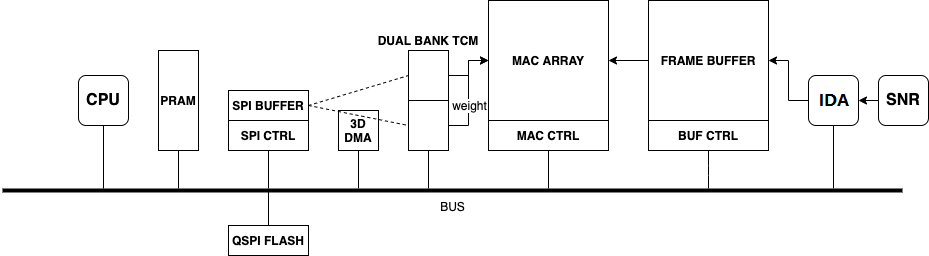
\includegraphics[width=15cm,height=4.5cm]{figures/bnn.png}
    \caption{总体架构图}
    \label{1}
\end{figure}
%TODO 各个模块的简述
在设计和建模过程中,假设从ISP输出的数据为我们人体肉眼可见的视频数据流。为了减少建模过程中的非相关设计,这里
的视频数据流假设为RGB888的格式。

\section{CIS数据通路}
%TODO 展示Stream datapath的传输方式 sof eof href
%TODO DL accelerator在数据通路中的作用
%TODO Fix Timing模块做数据同步,最后输出结果
CIS芯片的作用,就是将图像传感器接收到的信号,转为数字信号后传输给后端。一般来说,我们把CIS
芯片上的设计逻辑称为数据通路。图像数据通路一般由输入、数据处理和输出三个部分组成。通常地,这三个部分也具有各自不同的时钟域。
在输入时钟域中,RX模块接收从CMOS传感器输出的数据。由IDA模块的缓冲区暂存数据后向后一个时钟域输出同步数据。
在数据处理的时钟域中,深度学习运算模块将进行推理操作。
在输出时钟域中,FT(fix timing)模块将调整输出的时钟频率.TX模块负责以指定格式输出图像数据。  

\subsection{数据流的输入}
%TODO 
%   数据流的输入将由IDA(Input Data Adapter)模块处理。这个模块的主要作用是将Sensor输出的数据放到一个缓存区。
%   并将视频数据流的plck同步到数据流的时钟域。

这里假设从图像传感器输出的图像数据为224x224像素尺寸的图像。
视频数据流的输入需要参考流式设备的特性,合理的缓存大小和同步的时机是关键点。
对于卷积运算,缓存的行数大小应该大于等于卷积核的行数和列数之间的较大值。
例如,卷积核的尺寸为3x3时,缓存至少要保存3行数据。
如果,每帧图像的尺寸为224x224个像素点。
由RGB三个通道组成的每一帧都拆分成三个224x224x8比特。
那么需要给一个通道的一帧数据缓存的大小需要大于等于672个字节。


\section{深度学习神经网络运算单元}


% TODO CPU和GPU平台上的加速运算
在CPU和GPU平台上,SIMT和SIMD等技术被广泛地应用。
从字面上解释,SIMT是单指令多线程,而SIMD为单指令多数据流。


\subsection{影响因子和依据}
在开始设计深度学习神经网络的运算模块之前,本章节将提出一些影响设计的因素,并描述如何将这些因素考虑在内来帮助我们完成设计。
其中精准度、吞吐量、延迟、能效比和功耗,都是衡量深度学习神经网络运算的硬件单元的最重要因素。


% TODO 精确度 吞吐量和延迟 能效比和功耗
准确度是这类问题中最常见的一个指标。对于图像分类问题,准确度报告为正确分类图像的百分比,而对于目标检测问题,精度报告为平均准确度。
影响准确性的因素包括任务的难度和数据集。因此,准确度在建模的过程中将被用来验证设计的正确性。
吞吐量用于指示在给定时间段内可以处理的数据量或可以完成的任务的执行次数。高吞吐量通常是应用程序的关键。
延迟度量输入数据到达系统和生成结果之间的时间。低延迟对于实时交互应用程序(如虚拟现实、自主导航和机器人技术)是必要的。
吞吐量和延迟通常被认为是可以直接相互派生的。
一般的,在给定能量单位下可处理的数据量或完成任务的执行次数被称为能效比。




\subsection{基于脉动阵列的深度残差网络}
本文中将基于脉动阵列来实现深度残差网络。

%TODO ResNet18的Basic Block
%TODO x -> conv3x3 -> BN -> Relu -> conv3x3 -> BN ( + 入口的x)-> out -> Relu -> out
%TODO x -> conv7x7,stride=3,padding=3 -> BN -> 



%TODO 脉动阵列实现矩阵乘法的CMODEL
脉动阵列是1978年KUNG H T提出的一种应用在片上多处理器的体系结构。它是由多个相同的、结构简单的计算单元
以网状形式连接而成的,具有并行性、规律性和局部通信的特征。在深度残差网络ResNet18中,由5个卷积层组成,
除了第一个卷积层外,后4个卷积层都是由2个基础块组成。基础块的结构如下图x所示。其中的批量标准化和Relu函
数都可以设计专用的运算模块,而3x3的卷积运算可以通过脉动阵列来运算。


%REF KUNG H T, Leiserson C E. Systolic arrays(for VLSI)[C]. Sparse Matrix Proceedings 1978, Society for Industrial and Applied Mathematics, 1979.

脉动阵列的设计和C模型实现,可以分为两个部分:脉动阵列模块的顶层设计和处理单元的设计。
处理单元(PE)的寄存器:时钟、重置、同步清零、输入参数A、输入参数B、输出给下一级的A、输出给下一级的
B、输出P值。

\begin{table}[!hpt]
    \bicaption[PE的寄存器表]{PE的寄存器表}{Register Table Of PE}
    \label{tab:firstone}
    \centering
    \begin{tabular}{@{}lllr@{}} \toprule
        Type & Name & Description & Size \\ \midrule
        input  & CLK  & 输入PE模块的时钟信号 & 32b \\
        input  & RST  & 模块重置寄存器 & 16b \\
        input   & SCLR   & 同步清零寄存器 & 16b \\
        input   & A   & 输入参数A & 8b \\
        input   & B   & 输入参数B & 8b \\
        output   & Next\_A   & 输出到下一个PE的A & 8b \\
        output   & Next\_B   & 输出到下一个PE的B & 8b \\
        output & P & PE的运算结果P & 16b \\ \bottomrule
    \end{tabular}
  \end{table}

  

% \begin{table}[!hpt]
%     \caption[PE的寄存器表]{PE的寄存器表}{Register Table Of PE}
%     \label{tab:firstone}
%     \centering
%     \begin{tabular}Type & Name & Description & Size \\  \toprule
%       input & CLK  & 输入PE模块的时钟信号 & 32b \\ \midrule
%       input & RST  & 模块重置寄存器 & 16b \\
%       input & SCLR & 同步清零寄存器 & 16b \\
%       input & A & 输入参数A & 8b \\
%       input & B & 输入参数B & 8b \\
%       output & Next_A & 输出到下一个PE的A & 8b \\
%       output & Next_B & 输出到下一个PE的B & 8b \\
%       output & P & PE的运算结果P & 16b \\ \bottomrule
%     \end{tabular}
% \end{table}  



\section{存储}
%TODO 关于存储Multiple Bank的设计(状态机)
本设计中,专门对存储进行了优化,区分开了不同的RAM区域来存储不用的数据,主要由以下几个区域:存储输入和输出数据的
INRAM和OUTRAM、存储网络数据的NRAM、存储权重的WRAM、存储系统数据的SRAM以及存储临时数据的TRAM。拆分存储的设计
主要有以下两大好处:读写的带宽和避免冲突。
拆分存储之后,SRAM可以被调整为适当的读写宽度。假设输入和输出的宽度是$X_a \times K$字节,存储网络和权重数据的
NRAM和WRAM为$X_a \times X_a \times K$字节。如果是用CPU或GPU,且未做优化的情况下,处理器只能按照固定宽度读取
数据。

DRAM和SRAM
先进的存储技术可以降低高密度存储器(如DRAM)的访问能量。
例如,嵌入式DRAM(eDRAM)在芯片上提供高密度存储器,以避免关闭芯片电容的高能耗成本[97];eDRAM的密度比SRAM高2.85倍,能效比DRAM高321倍(DDR3)[93]。
与DRAM相比,eDRAM还提供了更高的带宽和更低的延迟。在DNN处理中,eDRAM可用于在芯片上存储数十兆字节的权重和激活,以避免芯片外访问,如DaDianNao[93]所示。
eDRAM的缺点是其密度低于片外DRAM,并且会增加芯片成本。
DRAM也可以使用硅通孔(TSV)堆叠在芯片顶部,而不是将DRAM集成到芯片本身。
这项技术通常被称为三维存储器,并已以混合存储立方体(HMC)[98]和高带宽存储器(HBM)[99]的形式商业化。
3-D内存提供了一个数量级的更高带宽,并且相对于现有的2-D DRAM,访问能量减少了5倍,因为TSV的电容低于典型的片外互连。
最近的工作探索了使用HMC以多种方式高效处理DNN。例如,Neurocube[100]将SIMD处理器集成到HMC的逻辑芯片中,使内存和计算更紧密地结合在一起。
Tetris[101]探讨了HMC与Eyeris空间架构和行固定数据流的结合使用。
它建议分配比片上存储器更多的计算区域(即更大的PE阵列和更小的全局缓冲区),以利用HMC的低能量和高吞吐量特性。它还调整数据流,以考虑HMC内存和更小的片上内存。
Tetris在使用传统2-D DRAM的基线系统上实现了1.5倍的能耗降低和4.1倍的吞吐量增加。

SRAM不是将内存放在计算附近,而是将计算放在内存中。
例如,乘法和累积操作可以直接集成到SRAM阵列的位单元中[102],如图36(a)所示。
在这项工作中,使用5位DAC将字线(WL)驱动到表示特征向量的模拟电压,而位单元存储二进制权重±1。
比特单元电流(IBC)实际上是特征向量的值和存储在比特单元中的权重的值的乘积;来自列中位单元的电流加在一起对位线(VBL)放电。
与从SRAM读取1位权重并单独执行计算相比,该方法可节省12倍的能量。
为了对抗电路的非理想性,DAC考虑了关于WL电压的非线性位线放电,并使用升压来组合易受设备变化影响的弱分类器,以形成强分类器[103]。

非易失性电阻存储器
乘法和累积操作也可以直接集成到高级非易失性高密度存储器中,方法是将其用作可编程电阻元件,通常称为忆阻器[105]。
具体地,如图36(b)所示,以电阻器的电导作为权重,以电压作为输入,以电流作为输出,执行乘法。
加法是通过将不同忆阻器的电流与基尔霍夫电流定律相加来完成的。这是权重固定数据流的最终形式,因为权重始终保持在适当的位置。
这种方法的优点包括:由于计算被嵌入内存中,从而减少了数据移动,因此降低了能耗;由于内存和计算可以以与DRAM类似的密度进行密集封装,因此增加了密度[106]。
非易失性电阻存储器器件有几种常见的候选器件,包括相变存储器(PCM)、电阻RAM(RRAM或ReRAM)、导电桥RAM(CBRAM)和自旋转移转矩磁RAM(STT-MRAM)[107]。
这些设备在耐久性(即可以写入多少次)、保留时间、写入电流、密度(即单元大小)、变化和速度方面有不同的权衡。
如[108]所述,使用非易失性电阻存储器进行处理有几个缺点。
首先,它受到前面描述的模拟处理的精度降低和ADC/DAC开销的影响。
第二,阵列尺寸受到连接电阻器件的导线的限制;具体而言,对于大型阵列(例如1k×1k),导线能量占主导地位,并且沿导线的红外压降会降低读取精度。
第三,对电阻器件进行编程的写入能量可能非常昂贵,在某些情况下需要多个脉冲。
最后,电阻器件还可能受到器件间和周期间变化的影响,在整个电导范围内具有非线性电导。


